\chapter{Théorème des résidus}
\section{Développement en série de Laurent}
Cette section est à connaître en totalité.
\subsection{Série de Taylor d'une application holomorphe}
Soit dans le plan complexe le disque ouvert $D$ de centre $z_0$ et de rayon
$r>0$. Le bord $\partial D$ est le cercle $\mathcal{C}$ de centre $z_0$ et de
rayon $r$ (voir \ref{Fi:Taylor}. Soit $f$ une application $\overline{D} \to
\mathbb{C}$ holomorphe dans $D$ et continue sur $\mathcal{C}$.
\begin{figure}
\scalebox{.68}{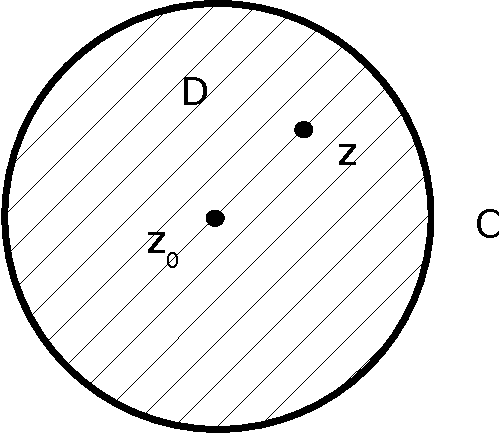
\includegraphics{images/taylor.pdf}}
\caption{Domaine D}\label{Fi:Taylor}
\end{figure}
En un point de $z \in D$, la formule de Cauchy permet d'écrire~:
\[
f(z) = \frac{1}{i2\pi}\int_{\mathcal{C}} \frac{f(u)}{u-z} du
\]
Soit, en faisant intervenir le point $z_0$~:
\[
f(z) = \frac{1}{i2\pi}\int_{\mathcal{C}} \frac{f(u)}{(u-z_0)-(z-z_0)} du =
\frac{1}{i2\pi}\int_{\mathcal{C}}
\frac{1}{u-z_0}\frac{f(u)}{1-\frac{z-z_0}{u-z_0}} du
\]
Pour $N \in \mathbb{N}$ fixé, on a~:
\[
\frac{1}{1-\frac{z-z_0}{u-z_0}} = \sum_{n=0}^N \left ( \frac{z-z_0}{u-z_0}
\right )^n + \left ( \frac{z-z_0}{u-z_0}
\right )^{N+1} \frac{1}{(u-z_0)-(z-z_0)}
\]
L'application $f$ étant par hypothèse continue sur le compact $\mathcal{C}$,
il existe un réel $M$ tel que $|f(z)|\leq M, z \in \mathcal{C}$. L'intégrale~:
\[
\int_{\mathcal{C}} \left ( \frac{z-z_0}{u-z_0}
\right )^{N+1} \frac{f(u)}{(u-z_0)-(z-z_0)} du 
\]
est bornée en module par~:
\[
\left ( \frac{|z-z_0|}{r}
\right )^{N+1} \frac{Mr}{r-|z-z_0|}
\]
Comme~:
\[
\left ( \frac{|z-z_0|}{r}
\right ) < 1
\]
On en déduit la convergence de la série~:
\[
f(z) = \frac{1}{i2\pi}\int_{\mathcal{C}}
\frac{f(u)}{u-z_0}\sum_{n \in \mathbb{N}} \left ( \frac{z-z_0}{u-z_0} \right )^n
du
\]
Par application de la formule de Cauchy~:
\[
\frac{1}{i2\pi} \int_{\mathcal{C}}
\frac{f(u)}{(u-z_0)^{n+1}} = \frac{f^{(n)}(z_0)}{n!}
\]
D'où finalement l'expression du développement en série de Taylor de $f$ en tout
point $z \in D$~:
\[
f(z)= \sum_{n\in \mathbb{N}} \frac{f^{(n)}(z_0)}{n!} (z-z_0)^n
\]
Il est clair que le développement en série de Taylor de $f$ dans $D$ est
unique.

\subsection{Développement au voisinage d'un point singulier isolé}
En utilisant les mêmes notations que dans la section précédente, on supposera
maintenant que $f$ est holomorphe dans l'ouvert $D- \{ z_0 \}$.
Soit $r_1$ vérifiant~:$r > r_1 > 0$. L'application $f$ est holomorphe dans
la couronne ouverte $\mathcal{C}$ de centre $z_0$, de rayon extérieur $r$ et de
rayon intérieur $r_1$. Le bord de cette couronne est la réunion des deux
cercles $\mathcal{C}_1, \mathcal{C}_2$ de centre $z_0$ et de rayons respectifs
$r$ et $r_1$. Le cercle $\mathcal{C}_1$ sera orienté positivement en sens
trigonométrique, le cercle $\mathcal{C}_2$ sera orienté en sens inverse
trigonométrique (le bord reçoit ainsi son orientation canonique). Par
application de la formule de Cauchy et en tenant compte de l'orientation de
$\mathcal{C}_2$, on obtient pour tout $z \in \mathcal{C}$~:
\[
f(z) = \frac{1}{i2 \pi} \int_{\mathcal{C}_1} \frac{f(u)}{u-z}du - \frac{1}{i2
\pi} \int_{\mathcal{C}_2} \frac{f(u)}{u-z}du
\]
La première intégrale de la partie droite se développe de la même façon que
précédemment et l'on obtient~:
\[
\frac{1}{i2 \pi} \int_{\mathcal{C}_1} \frac{f(u)}{u-z}du = \sum_{n \geq 0} a_n
(z-z_0)^n
\]
avec~:
\[
a_n = \frac{1}{i2\pi} \int_{\mathcal{C}_1} \frac{f(u)}{(u-z_0)^{n+1}}du
\]
\begin{rem}
Bien prendre garde à ne pas écrire $a_n=\frac{f^{(n)}(z_0)}{n!}$ car $f$ n'est
pas supposée holomorphe au voisinage de $z_0$.
\end{rem}
Pour la seconde intégrale, on utilisera l'expression suivante~:
\[
\frac{1}{z-u} = \frac{1}{(z-z_0)-(u-z_0)} = \frac{1}{z-z_0}\frac{1}{1-
\frac{u-z_0}{z-z_0}}
\]
En procédant de la même façon que pour la série de Taylor, et en remarquant que
pour $u \in \mathcal{C}_2$~:
\[
\left | \frac{u-z_0}{z-z_0} \right | < 1
\]
on obtient l'expression suivante~:
\[
- \frac{1}{i 2 \pi} 
\int_{\mathcal{C}_2} \frac{f(u)}{u-z}du = \sum_{n \geq 1} b_n
\frac{1}{(z-z_0)^n}
\]
avec~:
\[
b_n = \frac{1}{i2\pi} \int_{\mathcal{C}_2} (u-z_0)^{n-1}f(u) du
\]
Le développement correspondant~:
\[
f(z) = \sum_{n \geq 0} a_n
(z-z_0)^n + \sum_{n \geq 1} b_n (z-z_0)^{-n}
\]
s'appelle développement en série de Laurent de $f$ dans la couronne
$\mathcal{C}$.
Le développement en série de Laurent est unique.
On notera, avec les hypothèses faites sur $f$, que les coefficients
$(a_n),(b_n)$ ne dépendent pas du rayon intérieur $r_1$. On distinguera trois
cas~:
\begin{itemize}
  \item Les coefficients $(b_n)$ sont tous nuls. Dans ce cas, on peut prolonger
  $f$ analytiquement en $z_0$ en posant $f(z_0)=a_0$. 
  \item Les coefficients $(b_n)$ sont nuls à partir d'un certain rang. Soit $p$
  le plus petit entier tel que $b_p \neq 0$ et $\forall n > p, b_n = 0$.
  L'application $z \mapsto (z-z_0)^p f(z)$ admet un prolongement analytique en
  $z_0$. On dira dans ce cas que $z_0$ est un pôle d'ordre $p$.
  \item Dans les autres cas, on dira que $z_0$ est un point singulier essentiel.
\end{itemize}
\begin{rem}
L'unicité du développement en série de Laurent permet souvent de calculer les
coefficients $(a_n)$ ou $(b_n)$ à partir de développement connus. Par exemple,
dans une couronne centrée en $0$, on aura~:
\[
exp(z^{-1}) = 1 + \sum_{n \geq 1} \frac{1}{n!} z^{-n}
\]
d'où l'on déduit $a_0=1, a_n=0 , n > 0$ et $b_n=\frac{1}{n!}, n \geq 1$ dans ce
cas.
\end{rem}
\begin{rem}
Au voisinage d'un pôle d'ordre $p$, l'application $g \colon z \mapsto (z-z_0)^p
f(z)$ admet un prolongement analytique. on peut donc calculer son développement en
série de Taylor~:
\[
g(z) = \sum_{n \geq 0} c_n (z-z_0)^n
\]
avec~:
\[
c_n = \lim_{z \to z_0} \frac{1}{n!} g^{(n)}(z)
\]
Ceci permet d'évaluer facilement les termes $(b_n)$ du développement de $f$~:
\[
b_n = c_{p-n}
\]
\begin{defn}
Une application $f$ est dite méromorphe dans un ouvert $\Omega$ si elle ne
possède dans $\Omega$ pour seuls points singuliers des pôles.
\end{defn}
\end{rem}
\section{Théorème des résidus}
Les résultats de la section précédente permettent de développer une application
$f$ au voisinage d'un point singulier isolé $z_0$. On notera le lien existant
entre $b_1$ et l'intégrale de l'application sur le cercle intérieur d'une couronne
entourant le point singulier. Le coefficient $b_1$, en raison de son importance,
a reçu un nom particulier~: c'est le résidu de $f$ en $z_0$, noté $Res(f;z_0)$.

\begin{fthm}
Soit $\Omega$ un ouvert $1$-connexe et soit 
$\gamma$ un lacet de $\Omega$ . Soit $f$ une application holomorphe dans 
$\Omega-\{z_1, \dots z_n\}$ où les $z_i,i=1\dots n$ sont distincts deux à deux.
On~:
\[
\int_{\gamma} f(z) dz = i 2 \pi \sum_{j=1}^n Res(f;z_i)
\]
\end{fthm}

\begin{proof}
Il existe pour chaque $z_j$ une
couronne ouverte $\mathcal{C}_j$ de centre $z_j$ ne contenant aucun autre point
singulier. Le développement en série de Laurent sur chacune de ces couronnes
montre que~:
\[
Res_{z_j}f = \frac{1}{i 2 \pi} \int_{c_j} f(z) dz
\]
avec $c_j$ cercle intérieur de $\mathcal{C}_j$, orienté en sens
trigonométrique. L'application $f$ étant holomorphe dans $\Omega - \cup_{j=1}^n
D_j$ avec $D_j$ disque ouvert de centre $z_j$ et de bord $c_j$, on a~:
\[
\int_{\gamma} f(z) dz - \sum_{j=1}^n \int_{c_j} f(z)dz =0
\]
et le résultat s'en déduit.
\end{proof}
\begin{rem}
Le calcul pratique des résidus d'une application $f$ peut s'obtenir par
développement en série de Laurent. Dans le cas d'un pôle simple en $z_0$, on
retiendra que si $f(z)=p(z)/q(z)$, alors~:
\[
Res_{z_0}f = \frac{p(z_0)}{q^\prime(z_0)}
\]
Si on a affaire a un pôle d'ordre $p$, on utilisera la formule~:
\[
Res_{z_0}f = \lim_{z \to z_0} \frac{1}{(p-1)!}
\frac{d^{p-1}}{dz^{p-1}}[(z-z_0)f(z)]
\]
\end{rem}
Il existe comme toujours une forme utilisant la formule de Stokes:

\begin{fthm}
Soit $\Omega$ un domaine de bord un lacet simple régulier de classe $C^1$
par morceaux. Soit $f$ une application
holomorphe dans $\Omega-\{z_1, \dots z_n\}$ où les $z_i,i=1\dots n$ sont
distincts deux à deux, et continue sur $\partial \Omega$ On a~:
\[
\int_{\partial \Omega} f(z) dz = i 2 \pi \sum_{j=1}^n Res(f;z_i)
\]
\end{fthm}

Le théorème des résidus est la base du calcul des intégrales de chemin et permet
également d'évaluer de très nombreuses intégrales généralisées.
\begin{exercice}
Calculer les intégrales généralisées suivantes~:
\[
\begin{array}{l}
I_1 = \int_0^{+\infty} \frac{x^2 \cos(ax)}{1+x^4} dx , \quad a \in
\mathbb{R}\\
I_2 = \int_0^{+\infty} \frac{ \sin x}{x}dx
\end{array}
\]
\end{exercice}
\section{Calcul numérique}
Les développements en série de Laurent permettent souvent d'approcher numériquement une fonction inconnue ou très difficile à calculer par une fraction rationnelle complexe. Le site:
\url{http://dlmf.nist.gov/} recense de très nombreuses fonctions, avec des méthodes permettant de les calculer. On y trouvera des expressions sous formes de fractions continues, dont la troncature à un ordre fini donne une fraction rationnelle. Dans certains cas, une approximation rationnelle est beaucoup plus efficace qu'un développement en série de Taylor. 

On supposera dans la suite que la fonction $f$ que l'on souhaite approcher est connue de façon expérimentale, sous la forme d'un échantillon de couples de complexes $(z_i,w_i), i=0 \dots N-1$ avec $w_i = f\left(z_i\right)$. On recherchera une fraction rationnelle:
\[
\widetilde{f} \colon z \mapsto \frac{\sum_{k=0}^P a_k z^k}{\sum_{j=0}^Q b_j z^j}
\]
qui minimise l'erreur de calcul:
\[
\sum_{i=0}^{N-1} \left|w_i - \widetilde{f}(z_i)\right|^2
\] 
Sous cette forme, il est assez difficile de trouver le jeu de paramètres optimaux $(a_k),(b_j)$. Le problème sera donc reformulé comme la recherche des coefficients minimisant:
\[
\sum_{i=0}^{N-1} \left|w_i \sum_{j=0}^Q b_j z_i^j - 
\sum_{k=0}^P a_k z_i^k \right|^2
\] 
Ce problème est mal posé sous cette forme: rien ne change en effet si l'on multiplie les coefficients  $(a_k),(b_j)$ par un même nombre complexe. On lèvera cette indétermination en fixant un des coefficients à 1, typiquement $a_P$ ou $b_Q$ (on choisit ici de poser $a_P=1$). En se rappelant que la norme carrée d'un vecteur complexe s'écrit comme la somme des modules carrés de ses composantes, le critère précédent admet une formulation algébrique simple: il s'agit de trouver le vecteur complexe $v=(a_0, \dots,a_{P-1},b_0, \dots, b_Q)$ rendant minimum la norme carrée du vecteur:
\[
M v - 
\left(
\begin{array}{c}
z_0^P \\
z_1^P \\ 
\vdots \\ 
z_{N-1}^P
\end{array}
\right)
\]
avec $M$ la matrice:
\[
\left(
\begin{array}{cccccccc}
-1 & -z_0 & \dots & -z_0^{P-1} & w_0 & w_0 z_0 & \dots & w_0 z_0^Q
 \\
-1 & -z_1 & \dots & -z_1^{P-1} & w_1 & w_1 z_1 & \dots & w_1 z_1^Q \\
\vdots & \vdots & \vdots & \vdots &\vdots & \vdots & \vdots & \vdots  \\
-1 & -z_{N-1} & \dots & -z_{N-1}^{P-1} & w_{N-1} & w_{N-1} z_{N-1} & \dots & w_{N-1} z_{N-1}^Q
\end{array}
\right)
\]
On reconnaît un classique problème de résolution de système linéaire au sens des moindres carrés. L'objectif du cours n'étant pas l'étude des algorithmes d'algèbre linéaire, on se contentera d'utiliser une routine toute faite, disponible dans le module \texttt{numpy}, qu'il conviendra donc de charger. Voici le code correspondant:
\begin{verbatim}
# -*- coding: utf8 -*-
import math
import cmath
import numpy as np
from numpy.core.multiarray import dtype

#une classe très simple qui stocke des paires
class Pair:
    def __init__(self,p,q):
        self.first = p
        self.second = q


# Approximation d'une fonction par une fraction rationnelle
# au sens des moindres carrés 
class RationalSmoother:
    # constructeur pour l'approximation rationnelle
    # prend en paramètre les degrés du numérateur et du dénominateur
    # ainsi que la liste des échantillons, sous la forme de liste 
    # de paires
    # p: entier
    # q: entier
    # sample: liste de 'objets de type Pair
    def __init__(self,p,q,sample):
        self.p = p
        self.q = q
        #  creation de la matrice des échantillons
        m = np.zeros((len(sample),p+q+1),dtype=np.complex)
        # creation du second membre
        rhs = np.zeros((len(sample),1),dtype=np.complex)
        # iteration sur les lignes
        for i in range(len(sample)):
            m[i,0] = np.complex(-1.0,0.0)
            for j in range(p-1):
                m[i,j+1] = m[i,j] * sample[i].first
            rhs[i] = m[i,p-1] * sample[i].first
            m[i,p] = sample[i].second
            for j in range(q):
                m[i,p+1+j] = m[i,p+j] * sample[i].first
        # resolution du système
        self.coeff = np.linalg.lstsq(m, rhs)[0]
     # evaluation au point z
    def __call__(self,z):
        num = np.complex(1.0, 0.0)
        for i in range(self.p-1):
           num = num * z + self.coeff[self.p-i-1]
        den = self.coeff[p+q]
        for i in range(self.q):
           den = den * z + self.coeff[self.p+self.q-i]
        return num / den
# test sur la fonction sin
data = []
for i in range(20):
    ang = float(i)*math.pi*0.1
    z = complex(math.cos(ang),math.sin(ang))
    data.append(Pair(z,cmath.sin(z)))
p = 6
q = 2
rs = RationalSmoother(p,q,data)
for i in range(20):
    ang = float(i)*math.pi*0.1
    z = complex(math.cos(ang),math.sin(ang))
    print(cmath.sin(z), rs(z))
\end{verbatim}
\newpage
\leftline{\textbf{Un peu d'histoire \dots}}
\vskip 12pt
\begin{tabular}{ll}
\multicolumn{2}{l}{\textbf{Pierre Alphonse Laurent}} \\[10pt]
\begin{minipage}{0.2\linewidth}
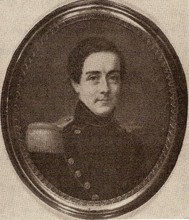
\includegraphics[scale=0.4]{images/Laurent.jpg}
\end{minipage}
&
\begin{minipage}{0.65\linewidth}
né le 18 juillet 1813 à Paris et mort le 2 septembre 1854. Polytechnicien à 19 ans, il commence une carrière militaire et participe aux expéditions de Mascart et de Tlemcen. A son retour, il fut chargé de travaux visant à l'agrandissement du port de Havre. Il exerçait son activité scientifique sur son temps libre. Il contribua en physique à la théorie des ondes et introduisit en analyse complexe le développement en série qui porte son nom. 
\end{minipage}\\
\multicolumn{2}{l}{\textbf{Brook Taylor}} \\[10pt]
\begin{minipage}{0.2\linewidth}
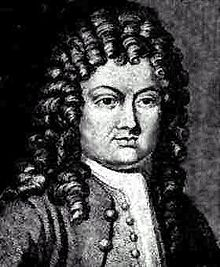
\includegraphics[scale=0.35]{images/Taylor.jpg}
\end{minipage}
&
\begin{minipage}{0.65\linewidth}
 Né à Edmonton (Londres) le 18 août 1685, et mort à Londres le 29 décembre 1731. Il invente l'intégration par parties et introduit le développement en série des applications différentiables. 
\end{minipage}
\end{tabular}
